
%(BEGIN_QUESTION)
% Copyright 2010, Tony R. Kuphaldt, released under the Creative Commons Attribution License (v 1.0)
% This means you may do almost anything with this work of mine, so long as you give me proper credit

En sikkerhetsenhet som ofte installeres på prosesskar med trykksatt gass, er en {\it Pressure Safety Valve} (PSV). I dette eksemplet beskytter en PSV en reaktortank mot ruptur ved for høyt internt gasstrykk. PSV-en er satt til å åpne («løfte») og avlaste tanken dersom internt trykk overstiger 95 PSI:

$$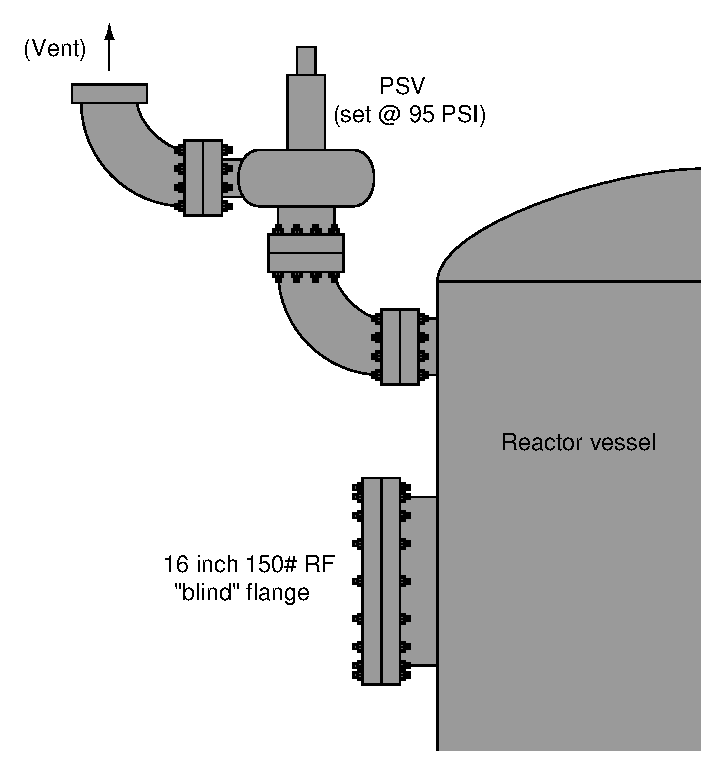
\includegraphics[width=15.5cm]{i00765x01.eps}$$

Beregn total kraft på en blindflens med 16 tommers diameter som sitter på siden av reaktoren ved PSV-ens løftetrykk. Beregn også belastningen fra denne kraften per bolt for de 20 boltene som holder flensen, med begge svar uttrykt i {\it pounds}. Bruk 15$1 \over 4$ tommer som effektiv diameter for blindflensen.

\vskip 10pt

$F_{total}$ = \underbar{\hskip 50pt} lb

\vskip 10pt

$F_{bolt}$ = \underbar{\hskip 50pt} lb


\vfil

\underbar{file i00765}
\eject
%(END_QUESTION)





%(BEGIN_ANSWER)

Dette er en vurdert oppgave -- ingen svar eller hint er gitt!

%(END_ANSWER)





%(BEGIN_NOTES)

Trykket inne i tanken virker mot flensens {\it effektive} areal. Med effektiv diameter 15.25 tommer blir effektivt areal 182.65 kvadrattommer. Ved 95 PSI på dette arealet blir kraften på flensen lik {\bf 17,352 pounds}.

\vskip 10pt

Hvis vi antar at alle 20 boltene som holder flensen tar lik andel av kraften, blir belastningen per bolt $1 \over 20$ av flenskraften, altså {\bf 867.6 pounds}.

%INDEX% Fysikk, væsker: trykk, kraft og areal
%INDEX% Fysikk, enheter og konvertering: trykk
%INDEX% Sikkerhet, overtrykksbeskyttelse: sikkerhetsventil

%(END_NOTES)


